% create a standalone latex file for generating a tikz figure.
% generate the following tikz visualization with two plots (added with \addplot), and several nodes. 
% 0. make the overall plot wide so that there is plenty of space.
% 1. create an x-axis and an y-axis.
% 2. the values along the x-axis should range from -5 to 5, and the values along the y-axis should range from 0 to 0.5.
% 3. first, plot the standard normal distribution curve on the graph, labeling it "normal (\mu=0, \sigma=1)", using a solid blue line, this has name path = mu0sigma1
% 4. second, plot the normal distribution curve on the graph with mean +1 and standard deviation 1, labeling it "normal (\mu=1, \sigma=1)", using a solid red line, this has name path = mu1sigma1
% 5. the legend position should be to the south of the plot, outside the plot area.
% 6. now we draw a vertical line that connects the x-axis to the mu0sigma1 curve at x = -0.3853205, this is node 101, no label value printed.
% 7. between the mu0sigma1 curve and the x-axis, we shade the area to the left of node 101 with a light blue color. this has name path = mu0sigma1area. We create a node outside of the shaded area, and label it as $P(H(h^{\text{base}}, d^{\text{base}}) \leq \zeta_{\text{good}}) = 0.350$, this points towards the shaded area mu0sigma1area. The label text should be fully visible in the plot. This node has node value 102.
% 8. between the mu1sigma1 curve and the x-axis, we shade the area to the left of node 101 with a light red color. this has name path = mu1sigma1area. We create a node outside of the shaded area, and label it as $P(H(h^{\text{base}}+1, d^{\text{base}}+1) \leq \zeta_{\text{good}}) = 0.083$, this points towards the shaded area mu1sigma1area. The label text should be fully visible in the plot. This node has node value 101.
% 9. We draw an extra x-axis tic at the x position of node 101. we then create a node with the value of -0.3853205 to 2 decimals, printed below the x-axis below the tic mark, and with an arrow pointing to the tic mark. This new node is named node 203. The label text should be fully visible in the plot. 

\documentclass{article}
\usepackage{geometry}
\geometry{
	a4paper,
	noheadfoot=true,
	left=1.0in,
	right=1.0in,
	top=1.0in,
	bottom=1.0in
}
\usepackage{amsmath}
\usepackage{float}
\usepackage{pgfplots}
\usepackage{subcaption}
\pgfplotsset{compat=1.17}
\usepgfplotslibrary{fillbetween}
\usetikzlibrary{decorations.pathreplacing}

\begin{document}

\begin{figure}[H]
    \centering
    \captionsetup{width=1.0\textwidth}
	\caption{Illustration of the identification of latent health thresholds and marginal effects given elicited subjective health probabilities across input scenarios and health status levels.}
	\label{fig:vert}
	\begin{subfigure}[t]{1.0\textwidth}
        % Sub-caption
        \centering
    		\caption{Baseline subjective health probabilities and thresholds}	
        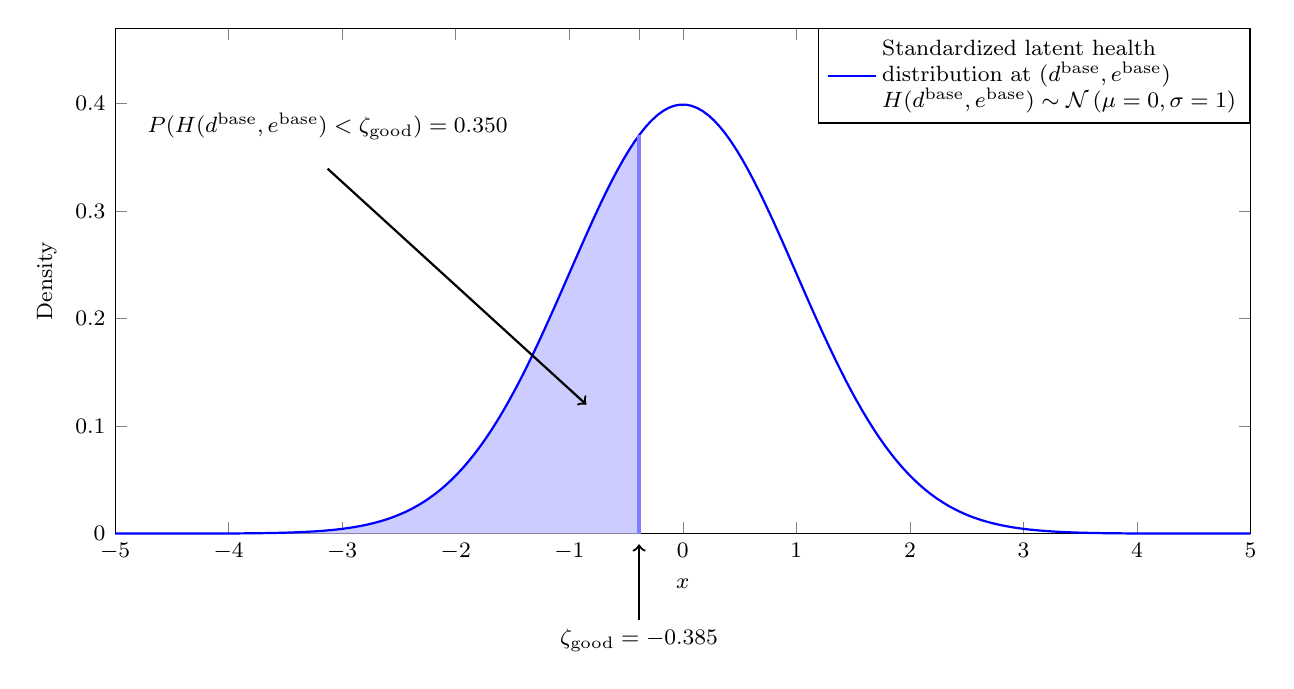
\begin{tikzpicture}
            \begin{axis}[
                width=16cm,
                height=8cm,
                font=\footnotesize,
                xlabel={$x$},
                ylabel={Density},
                xmin=-5, xmax=5,
                ymin=0, ymax=0.47,
                samples=200,
                domain=-5:5,
                legend style={at={(1.0, 1.0)}, anchor=north east, align=left},
                extra x ticks={-0.3853205},
                extra x tick labels={},
                clip=false
            ]
            
            % Plot standard normal distribution
            
            \addplot[blue, thick, name path=mu0sigma1] {1/sqrt(2*pi)*exp(-0.5*x^2)};
            \addlegendentry{
                Standardized latent health\\
                distribution at $(d^{\text{base}}, e^{\text{base}})$\\
                $H(d^{\text{base}}, e^{\text{base}}) \sim \mathcal{N}\left(\mu=0, \sigma=1\right)$
                }
            % Create path for x-axis
            \path[name path=axis] (axis cs:-5,0) -- (axis cs:5,0);
            
            % Shade area under mu0sigma1 to the left of x=-0.3853205
            \addplot[blue!20, name path=mu0sigma1area] fill between[of=mu0sigma1 and axis, soft clip={domain=-5:-0.3853205}];
            
            % Draw vertical line at x=-0.3853205 (node 101)
            \draw[solid, blue!50, very thick] (axis cs:-0.3853205,0) -- (axis cs:-0.3853205,{1/sqrt(2*pi)*exp(-0.5*(-0.3853205)^2)});
            
            % Node 102 for mu0sigma1 area
            \node[anchor=north west, align=left] at (axis cs:-4.8,0.40) (102) {
            % \node[anchor=north west, align=left] at (axis cs:-4.7, 0.50) (102) {
                % Elicit baseline $(d^{\text{base}}, e^{\text{base}})$ subjective\\ 
                % probability of less than good health: \\
                $P(H(d^{\text{base}}, e^{\text{base}}) < \zeta_{\text{good}}) = 0.350$\\
                % Given normalization, identify\\
                % latent health threshold for\\
                % good health: $\zeta_{\text{good}}=-0.385$.
                };
            \draw[->, thick] ( [xshift=0.0cm] 102.south) -- (axis cs:-0.85,0.12);
            
            
            % \draw[densely dashdotted, blue, very thick] (axis cs:0,0) -- (axis cs:0,{1/sqrt(2*pi)*exp(-0.5*(0)^2)});
            
            % Node 203 for x-axis label
            \node[anchor=north] at (axis cs:-0.3853205,-0.08) (103) {$\zeta_{\text{good}} = -0.385$};
            \draw[->, thick] (103) -- (axis cs:-0.3853205,-0.01);
            
            \end{axis}
        \end{tikzpicture}
    \end{subfigure}	
        
	\par\smallskip % this line generates two rows
    
	\begin{subfigure}[t]{1.0\textwidth}
	    % Sub-caption
	    \centering
        \caption{Subjective health probabilities at alternative input scenarios and marginal effects}   
            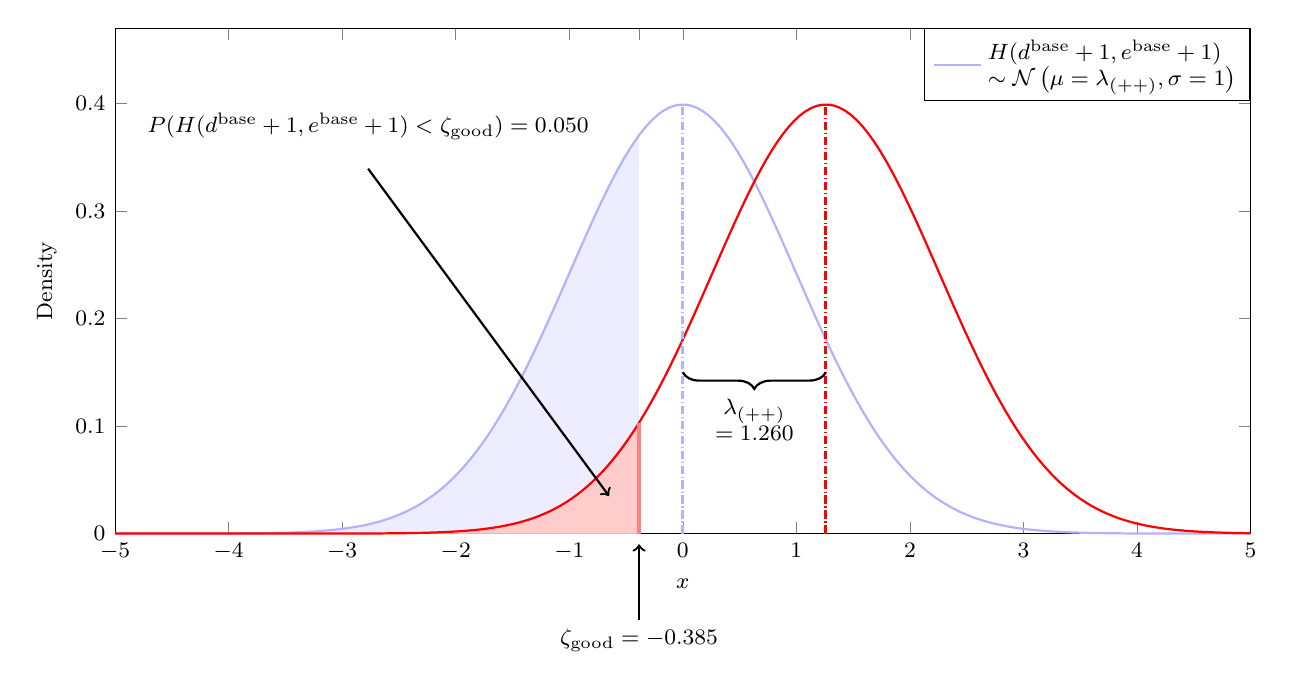
\begin{tikzpicture}
            \begin{axis}[
                width=16cm,
                height=8cm,
                font=\footnotesize,
                xlabel={$x$},
                ylabel={Density},
                xmin=-5, xmax=5,
                ymin=0, ymax=0.47,
                samples=200,
                domain=-5:5,
                legend style={at={(1.0, 1.0)}, anchor=north east, align=left},
                extra x ticks={-0.3853205},
                extra x tick labels={},
                clip=false
            ]
            
            
            % Plot standard normal distribution
            \addplot[blue!30, thick, name path=mu0sigma1] {1/sqrt(2*pi)*exp(-0.5*x^2)};
            % \addlegendentry{
            %     $H(d^{\text{base}}, e^{\text{base}}) \sim \mathcal{N}\left(\mu=0, \sigma=1)\right)$
            %     }
            
            % Plot normal distribution with mu=1, sigma=1
            \addplot[red, thick, name path=mu1sigma1] {1/sqrt(2*pi)*exp(-0.5*(x-1.259533)^2)};
            \addlegendentry{
                $H(d^{\text{base}}+1, e^{\text{base}}+1)$\\
                $\sim \mathcal{N}\left(\mu=\lambda_{\left(++\right)}, \sigma=1\right)$
                }
            
            
            % Create path for x-axis
            \path[name path=axis] (axis cs:-5,0) -- (axis cs:5,0);
            
            % Shade area under mu0sigma1 to the left of x=-0.3853205
            \addplot[blue!07, name path=mu0sigma1area] fill between[of=mu0sigma1 and axis, soft clip={domain=-5:-0.3853205}];
            
            % Shade area under mu1sigma1 to the left of x=-0.3853205
            \addplot[red!20, name path=mu1sigma1area] fill between[of=mu1sigma1 and axis, soft clip={domain=-5:-0.3853205}];
            
            % Draw vertical line at x=-0.3853205 (node 101)
            \draw[solid, red!50, very thick] (axis cs:-0.3853205,0) -- (axis cs:-0.3853205,{1/sqrt(2*pi)*exp(-0.5*(-0.3853205-1.259533)^2)});
            
            % % Node 102 for mu0sigma1 area
            % \node[anchor=east] at (axis cs:-1,0.425) (202) {$P(H(d^{\text{base}}, e^{\text{base}}) \leq \zeta_{\text{good}}) = 0.350$};
            % \draw[->, thick] ( [xshift=1cm] 202.south) -- (axis cs:-0.85,0.15);
            
            % Node 101 for mu1sigma1 area (note: description says node value 101)
            \node[anchor=north west, align=left] at (axis cs:-4.8,0.40) (202) {
            % \node[anchor=north west, align=left] at (axis cs:-4.8,0.52) (202) {
                % Elicit scenario-specific ($d^{\text{base}}+1, e^{\text{base}}+1$)\\
                % subjective probability of less than good health: \\
                $P(H(d^{\text{base}}+1, e^{\text{base}}+1) < \zeta_{\text{good}}) = 0.050$\\
                % Given $\zeta_{\text{good}}$ and the same uncertainty\\
                % distribution ($\sigma=1$) identify\\
                % the marginal shift in\\
                % latent health: $\lambda_{\left(++\right)}=1.260$\\
                };
            \draw[->, thick] ([xshift=0.0cm, yshift=+0cm] 202.south) -- (axis cs:-0.65,0.035);
            
            % draw a node 
            \draw[densely dashdotted, blue!30, very thick] (axis cs:0,0) -- (axis cs:0,{1/sqrt(2*pi)*exp(-0.5*(0)^2)});
            \draw[densely dashdotted, red, very thick] (axis cs:1.259533,0) -- (axis cs:1.259533,{1/sqrt(2*pi)*exp(-0.5*(0)^2)});
            % draw a underbrace between the two dashdotted lines
            \draw[decorate,decoration={brace,mirror,amplitude=6pt},thick,align=center]
                (axis cs:0,0.15) -- (axis cs:1.259533,0.15) node[midway,below=6pt] {
                    $\lambda_{\left(++\right)}$\\
                    $=1.260$
                    };
            
            % solve for lambda, such that:
            % qnorm(zeta, mean=lambda, sd=1) = 0.15
            
            % We have:
            % F_Y(zeta) = P(Y <= zeta) = prob2
            % Y = X + lambda
            
            % Therefore:
            % F_Y(zeta)
            % = P(Y <= zeta) 
            % = P(X + lambda <= zeta)
            % = P(X <= zeta - lambda)
            % = F_X(zeta - lambda)
            % = prob2
            
            % zeta - qnorm(prob2)
            % zeta = qnorm(prob1)
            
            
            % Node 203 for x-axis label
            \node[anchor=north] at (axis cs:-0.3853205,-0.08) (203) {$\zeta_{\text{good}} = -0.385$};
            \draw[->, thick] (203) -- (axis cs:-0.3853205,-0.01);
            
            
            \end{axis}
            \end{tikzpicture}
    		
	\end{subfigure}    
	\par\smallskip
    \parbox[t]{1.0\textwidth}{\footnotesize \emph{Note:}
    Next period latent health is a random variable. 
    The latent health random variable at baseline input levels is $H(d^{\text{base}}, e^{\text{base}})$. 
    The latent health random variable given increases in both input levels is 
    $H(d^{\text{base}}+1, e^{\text{base}}+1)$.
    We elicit subjective probabilities that next period latent health is worse than ``good'' at the baseline and alternative input scenarios.
    We assume that latent health is a mixture of normals (in this case one normal).
    Since the scale and location of latent variables can not be identified, we normalize $H(d^{\text{base}}, e^{\text{base}}) \sim \mathcal{N}\left(\mu=0, \sigma=1\right)$.
    The normalized latent threshold for good health, $\zeta_{\text{good}}$, can be identified by inverting the survey-elicited cumulative probability of having less than good health: 
    $\Phi^{-1}\left(P\left(H\left(d^{\text{base}}, e^{\text{base}}\right) < \zeta_{\text{good}} \right)\right) = \zeta_{\text{good}}$. 
    The marginal effect of increasing inputs is $\lambda_{\left(++\right)}$, where $\lambda_{\left(++\right)}$ provides a mean-shift of the baseline latent health random variable: $H(d^{\text{base}}+1, e^{\text{base}}+1) = H(d^{\text{base}}, e^{\text{base}}) + \lambda_{\left(++\right)}$.
    The marginal effect can be identified as the difference of inverted cdfs:
    We have $
    P\left(H\left(d^{\text{base}}+1, e^{\text{base}}+1\right) < \zeta_{\text{good}} \right) = 
    P\left(H\left(d^{\text{base}}, e^{\text{base}}\right) + \lambda_{\left(++\right)} < \zeta_{\text{good}} \right) = 
    \Phi\left(\zeta_{\text{good}} - \lambda_{\left(++\right)}\right)
    $, and hence $
    \lambda_{\left(++\right)} = \zeta_{\text{good}} - 
    \Phi^{-1}\left(
        P\left(H\left(d^{\text{base}}+1, e^{\text{base}}+1\right) < \zeta_{\text{good}} \right)
    \right)
    $.
    }
\end{figure}
\end{document}